\subsection{The Mean Value Theorem}

\ex{1}
\begin{proof}
    Since $f'$ is assumed continuous on a compact set $[a,b]$
    then by the extreme value \Thm there exist $x_0, x_1 \in [a,b]$
    s.t. 
    \begin{align*}
        f(x_0) \leq f(x) \leq f(x_1)
    \end{align*}
    for all $x\in [a,b]$.

    Since $f$ is differential on $[a,b]$ then by MVT
    for $x<y$ with $x,y\in [a,b]$
    \begin{align*}
        f'(c) = \frac{f(y)-f(x)}{y-x} 
    \end{align*}
    for some $c \in (x,y)$. But $f'(x_0) \leq f'(c) \leq f'(x_1)$
    so 
    \begin{align*}
        f'(x_0) \leq  \frac{f(y)-f(x)}{y-x} \leq f'(x_1) 
    \end{align*}
    Choose $M = \max\{|f(x_0)| ,|f(x_0)|\}$ so that 
    \begin{align*}
        |\frac{f(y)-f(x)}{y-x}| \leq M
    \end{align*}
    Since $x,y$ where arbitrary then $f$ must be lipschitz.
\end{proof}

\ex{2}
\begin{proof}
    By \Ex{1} $f$ is lipschitz so 
    \begin{align*}
        |\frac{f(y)-f(x)}{y-x}| \leq M
    \end{align*}
    for some $M>0$.
    However, since the deritvative is always bounded by unity 
    then 
    \begin{align*}
        |f'(c)| = |\frac{f(y)-f(x)}{y-x}| < 1 < s
    \end{align*}
    where $0<s<1$ so 
    \begin{gather*}
        |\frac{f(y)-f(x)}{y-x}| \leq s
        \Rightarrow |f(y)-f(x)| \leq s |y-x|
    \end{gather*}
    for some $0<s<1$.
\end{proof}

\ex{3}
\begin{enumerate}[label=(\alph*)]
    \item 
    Let's define $g(x)=h(x)-x$. In terms of $g$ our 
    goal is find a root.
    Now 
    \begin{gather*}
        g(0)=1 \\
        g(1)=1 \\
        g(3) = -1
    \end{gather*}
    $g$ is continuous so by IVT there exists $d\in (0,3)$
    s.t. 
    \begin{align*}
        g(d)=0
    \end{align*}
    This implies $h(d)=d$ as reequired.

    \item
    Sicne $h$ is differentiable on $[0,3]$ then by MVT 
    $\exists$ $c\in (0,3)$ s.t. 
    \begin{align*}
        h'(c) = \frac{h(3)-h(0)}{3} = \frac{1}{3} 
    \end{align*}

    \item
    For simplicity, let's define 
    \begin{align*}
        g(x) = h(x) - \frac{1}{4}x
    \end{align*}
    then 
    \begin{gather*}
        g(0)=1 \\
        g(1)=1.75 \\
        g(3) = 1.25
    \end{gather*}
    Now the end points do not occur at the end points $0,3$
    since we know $g(1)>g(0),g(3)$. Since $g$ is a continuous 
    function on a compact set then by the extreme value \Thm
    there exist $x_0, x_1 \in [0,3]$ s.t. 
    \begin{align*}
        g(x_0) \leq g(x) \leq g(x_1)
    \end{align*}
    so $x_1 \in (0,3)$. Hence, by the interior extremum \Thm 
    we know 
    \begin{gather*}
        g'(x_1) = 0 \\
        \Rightarrow g'(x_1) = h'(x) - 1/4 = 0 \\
        \Rightarrow h'(x) = 1/4
    \end{gather*}
\end{enumerate}

\ex{4}
\begin{enumerate}[label=(\alph*)]
    \item 
    \begin{proof}
        Let
        \begin{align*}
            h(x) = [f(b)-f(a)]g(x)-[g(b)-g(a)]f(x)
        \end{align*}
        Since $h$ is differentiable on $[a,b]$ then 
        by MVT there exists $c\in (a,b)$ s.t. 
        \begin{align*}
            h'(c) = \frac{h(b)-h(a)}{b-a}
        \end{align*}
        Now 
        \begin{align*}
            h(b) &= [f(b)-f(a)]g(b) - [g(b)-g(a)]f(b) \\
                &= g(a)f(b)-f(a)g(b)
        \end{align*}
        Similarly,
        \begin{align*}
            h(a) &= [f(b)-f(a)]g(a) - [g(b)-g(a)]f(a) \\
                &= f(b)g(a)-g(b)f(a)
        \end{align*}
        So 
        \begin{gather*}
            h(b)-h(a) = 0 \\
            \Rightarrow h'(c)=0 \\
            \Rightarrow (f(b)-f(a))g'(c) = f'(c)(g(b)-g(a))
        \end{gather*}
        If $g'$ is never zero then $g(a) \neq g(b)$ and the 
        result can be rewritten as  
        \begin{align*}
            \frac{f'(c)}{g'(c)} = \frac{f(b)-f(a)}{g(b)-g(a)}
        \end{align*}
    \end{proof}

    \item
    For clarity we will denote our parametric equations as
    $x(t), y(t)$ for the x- and y-coordinate respectively.

    Assuming $t\in [a,b]$ then the slope between the 
    end points is 
    \begin{align*}
        \text{slope of endpoints} = \frac{y(b)-y(a)}{x(b)-x(a)}
    \end{align*}
    The tangent vector to the curve at any point is 
    given by 
    \begin{align*}
        \lim_{h\rightarrow 0} \frac{\vec r(t+h)-\vec r(t)}{h} = (x'(t),y'(t))
    \end{align*}
    where $\vec r(t)=(x(t),y(t))$.
    The gradient of the tangent vector is 
    \begin{align*}
        \text{gradient of tangent vector} = \frac{y'(t)}{x'(t)}
    \end{align*}
    The generalized IVT is saying 
    \begin{align*}
        \text{slope of endpoints} = \text{gradient of tangent vector}
    \end{align*}
    at some $t\in (a,b)$.

    \begin{figure}
        \centering
        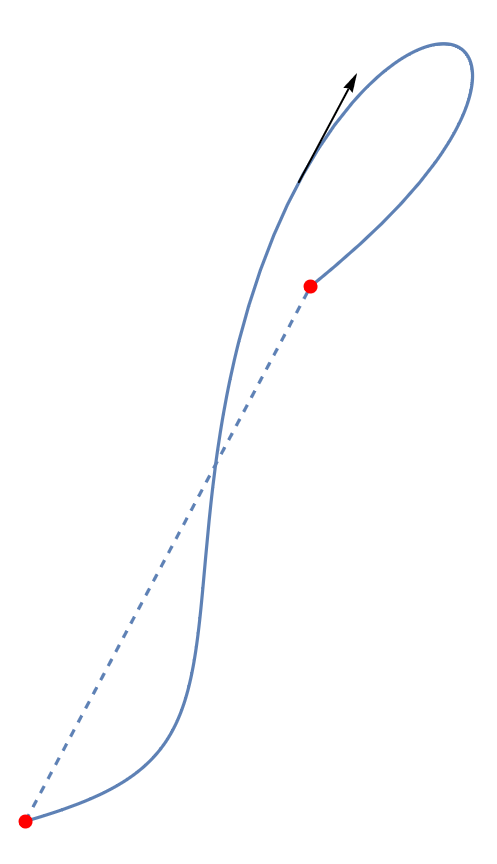
\includegraphics[width=.2\textwidth]{5 The Derivative/Exercise 5.3.4/Exercise 5.3.4 (b).png}
        \caption{\Ex{4} (b) \label{fig:Ex_3_4_b}}
    \end{figure}
    An illustration of this result is shown in figure \ref{fig:Ex_3_4_b}.
\end{enumerate}

\ex{5}
\begin{proof}
    Let $h(x)=f(x)-x$ then we are trying to find where 
    $h(x)$ is zero. Now since $f'(x)\neq 1$ then 
    $h'(x) = f'(x)-1 \neq 0$. For any $x,y \in [a,b]$ with 
    $x<y$
    \begin{align*}
        \frac{h(y)-h(x)}{y-x} = h'(c) \neq 0
    \end{align*}
    for some $c \in (x,y)$ which implies $h(y) \neq h(x)$ for 
    $x\neq y$. Suppose there is one fixed point at $d \in [a,b]$,
    then $h(d)=0$ and $0=h(d)\neq h(y)$ so there are no more fixed 
    points.
\end{proof}

\ex{6}
\begin{proof}
    Let's define $h(x)=g(x)-x$, then in terms of
    $h$ we need to show $h(d) \Leftrightarrow h'(1)>0$. 

    The conditions assumed on $g$ translate to $h$ as:
    \begin{gather*}
        h(0)>0 \\
        h(1) = g(1)-1=0 \\
        h''(x) > 0
    \end{gather*}

    $(\Rightarrow)$ Suppose $h(d)=0$ for som e$d\in (0,1)$, then 
    $h''$ positive implies $h'$ is strcitly monotonic increasing.
    So if $h(d)=0$ then $h(x)>0$ for $x>d$. Hence $h'(1)>0$.

    $(\Leftarrow)$ Suppose $h'(1)>0$. Now $h(0)>0$ and $h(1)=0$. Since 
    $h'$ is strcitly increasing then $h'(0)<0$. 
    So we have $h'(0)<0$ and $h'(1)>0$ and since $h'$ is continuous then 
    by the IVT there exists $d\in (0,1)$ s.t. $h(d)=0$.
\end{proof}

\ex{7}
\begin{enumerate}[label=(\alph*)]
    \item 
    \begin{proof}
        $(\Rightarrow)$ Suppose $f$ is increasing. 
        Since $f$ is differentiable on $(a,b)$ then 
        \begin{align*}
            f'(c) = \lim_{x\rightarrow c} \frac{f(x)-f(c)}{x-c}
        \end{align*}
        exists for any $c\in (a,b)$.
        Hence, consider sequence $(x_n)\rightarrow c$ where 
        $(x_n)\in (a,b)$ and $x_n<c$ for all $n\in \mathbb{N}$.
        Hence, 
        \begin{align*}
            x_n - c < 0 \Rightarrow f(x_n) f(c) \leq 0
        \end{align*}
        so 
        \begin{align*}
            \frac{f(x_n)-f(c)}{x_n-c} > 0
        \end{align*}
        for all $n\in \mathbb{N}$.
        By the order limit \Thm this implies $f'(c)\geq 0$.
        Since $c$ was arbitrary then $f'(x)\geq 0$ for $x\in(a,b)$.
    
        $(\Leftarrow)$ Suppose $f'(x)\geq 0$ for $x\in (a,b)$.
        For any $x,y\in (a,b)$ s.t. $x<y$ then by the MVT
        \begin{align*}
            f'(c) = \frac{f(y)-f(x)}{y-x} \geq 0
        \end{align*}
        for some $c\in (x,y)$.
        However this implies $f(y)>f(x)$. Since $x,y$ where 
        arbitrary then $f$ is increasing.
    \end{proof}

    \item
    From our previous studies we know $x^2 \sin(1/x)$ is
    differentiable on $\mathbb{R}$. Hence, the derivative of 
    $g$ is given by
    \begin{align*}
        g'(x) = \begin{cases}
            1/2 + 2x \sin(1/x) - \cos(1/x) & x\neq 0 \\
            1/2 & x=0
        \end{cases}
    \end{align*}
    To show $g$ is not increasing on any open interval we need to show 
    $g'(x)<0$ for at least a single $x$ in every open interval around zero.
    
    For some interval $(-\varepsilon, \varepsilon)$, assume $\varepsilon<1/8$,
    then $-1/4 \leq 2x\sin(1/x) \leq 1/4$ and $-1 \leq \cos(1/x) \leq 1$ so 
    since $\sin$ and $\cos$ are $\pi/2$ out of phase we know peaks will meet 
    with trophs and vice versa so
    \begin{align*}
        -3/4 \leq 2x\sin(1/x) - \cos(1/x) \leq 3/4
    \end{align*}
    so $g$ is not strcitly increasing since every open interval around zero of
    $g'$ is not strictly non-negative then $g$ is not increasing. 
\end{enumerate}

\ex{8}
\begin{proof}
    Suppose $g'(c)\neq 0$, without loss of generality assume 
    $g'(c)>0$. For $\varepsilon=g'(c)/2$ there exists $\delta>0$
    s.t. 
    \begin{align*}
        0<|x-c|<\delta \Rightarrow |\frac{g(x)-g(c)}{x-c}-g'(c)| < g'(c)/2
    \end{align*}
    This implies 
    \begin{align*}
        0<g'(c)/2 < \frac{g(x)-g(c)}{x-c} < 3g'(c)/2
    \end{align*}
    Multiplying through by $x-c$
    \begin{align*}
        \begin{cases}
            g(x)-g(c) > 0 & x < c \\
            g(x)-g(c) < 0 & x > c
        \end{cases} \\
        \Rightarrow \begin{cases}
            g(x) > g(c) & x < c \\
            g(x) < g(c) & x > c
        \end{cases}
    \end{align*}
    so $g(x)\neq g(c)$ for $c \in V_\delta(c)$ excluding 
    $x=c$ ofcourse.
\end{proof}

\ex{9}
\begin{proof}
    Choose $M>0$,
    since $\lim g(x) = 0$ then there exists $\delta_1>0$ s.t. 
    \begin{align*}
        0<|x-c|<\delta_1 \Rightarrow |g(x) - g(c)| < \frac{L-1}{M}
    \end{align*}
    Since $\lim f(x)=L$ then there exists $\delta_1>0$ s.t. 
    \begin{align*}
        0<|x-c|<\delta_2 \Rightarrow |f(x) - f(c)| < 1 \Rightarrow L-1<f(x)<L+1
    \end{align*}
    so for $\delta=\min\{\delta_1,\delta_2\}$
    \begin{align*}
        0<|x-c|<\delta \Rightarrow |\frac{f(x)}{g(x)}| > |\frac{L-1}{(L-1)/M}| > M
    \end{align*}
    Hence, $f(x)/g(x) \rightarrow \infty$
\end{proof}

\ex{10}
Assume $f$ is bounded by $M$ i.e. $f(x)<M$. Since 
$\lim g(x) = \infty$ then for $\varepsilon>0$ there exists 
$\delta>0$ s.t. 
\begin{align*}
    0<|x-c|<\delta \Rightarrow |g(x)|>\frac{M}{\varepsilon}
\end{align*}
This implies 
\begin{align*}
    |\frac{f(x)}{g(x)}| < \varepsilon
\end{align*}

\ex{11}
\begin{proof}
    $\lim f'(x)/g'(x)=L$ implies that for $\varepsilon>0$ 
    there exists $\delta>0$ s.t. 
    \begin{align*}
        0<|x-a|<\delta \Rightarrow |\frac{f'(x)}{g'(x)}-L|\varepsilon
    \end{align*}
    Since $f,g$ are differentiable on an interval containing $a$ then 
    $f,g$ are differentiable on the interval $[a,x]$ where $a<x<a+\delta$.
    Then by the generalized MVT 
    \begin{align*}
        (f(x)-f(a))g'(c) = (g(x)-g(a))f'(c)
    \end{align*}
    Since $g(a)=f(a)=0$ then 
    \begin{align*}
        f(x)g'(c) = g(x)f'(c)
    \end{align*}
    for some $c\in (a,x)$.
    However, $c,x\in V_\delta(a)$ so 
    \begin{align*}
        \varepsilon>|\frac{f'(c)}{g'(c)}-L|=|\frac{f'(x)}{g'(x)}-L|
    \end{align*}
    Since $x\in V_\delta(a)$ was arbitrary then $|\frac{f'(x)}{g'(x)}-L|<\varepsilon$
    for any $x\in V_\delta(a)$.
\end{proof}

\ex{12}
\begin{proof}
    Since $f',g'$ are continuous as $a$ then 
    \begin{align*}
        \lim_{a\rightarrow a}\frac{f'(x)}{g'(x)} &= \frac{f'(a)}{g'(a)} \\
        &= \frac{\lim_{x\rightarrow a}\frac{f(x)-f(a)}{x-a}}{\lim_{x\rightarrow a}\frac{g(x)-g(a)}{x-a}} \\
        &= \lim_{x\rightarrow a} \frac{\frac{f(x)-f(a)}{x-a}}{\frac{g(x)-g(a)}{x-a}} \\  
        &= \lim_{x\rightarrow a} \frac{f(x)}{g(x)}    
    \end{align*}
\end{proof}

\ex{13}
Since $f,g$ are continuous at $a$ then 
\begin{gather*}
    0=\lim_{x\rightarrow 0} f(x)=  f(\lim_{x\rightarrow 0} x) = f(0) \\
    0=\lim_{x\rightarrow 0} g(x)=  g(\lim_{x\rightarrow 0} x) = g(0)
\end{gather*}